% ------------------------------------------------------------------------------------------
% Modelo de qualificação para o PPGEE da PUCRS.
% Essa é uma versão atualizada por mim de uma primeira versão criada pela Nathalia Bianchini.
% O modelo foi criado e atualizado no ShareLatex.com e está sujeito a implementações futuras.
% Quaisquer problemas ou sugestões utilize o fórum de Issues do GitHub.
% Sinta-se livre para utilizar como bem entender.
%------------------------------------------------------------------------------------------

% ****************************************
% DEFINICOES GERAIS DO LAYOUT DO TRABALHO
\documentclass[11pt]{article}
\usepackage[utf8]{inputenc}
\usepackage{fontenc}
\usepackage{tikz}
\usepackage{pslatex}
\usepackage{setspace}
\usepackage{sectsty}
\usepackage{graphicx}
\usepackage{subcaption}
\captionsetup[subfigure]{font=scriptsize,labelfont=scriptsize}
\usepackage{eso-pic}
\usepackage{natbib}
\renewcommand\bibsection{\section{\refname}}
\usepackage{floatrow}
\usepackage{fancyhdr}
\usepackage{fancyref}
\usepackage{placeins}
\usepackage[font=footnotesize]{caption}
\usepackage{indentfirst} % Identa o primeiro parágrafo
\usepackage[top=2cm,bottom=6.15cm,left=3.17cm,right=3.49cm,footskip=3cm,headsep=0.1cm]{geometry}
\usepackage{multirow} %tables
\usepackage{amsmath}
\usepackage{nccmath}
\makeatother
\usepackage{colortbl}
\usepackage{enumitem}
\allowdisplaybreaks
\setlist{nosep}

%Cria links para as referências
\usepackage{csquotes}
\usepackage{hyperref}
\hypersetup{hidelinks}
\usepackage{url}
\urlstyle{same}

%Espaçamento das sessões e tamanho da fonte
\usepackage{titlesec}
\sectionfont{\fontsize{12}{15}\selectfont}
\subsubsectionfont{\fontsize{12}{15}\selectfont}
\titlespacing{\section}{0cm}{0.42cm}{0cm}
\titlespacing{\subsection}{0cm}{0.42cm}{0cm}
\titlespacing{\subsubsection}{0cm}{0.42cm}{0cm}
\renewcommand{\bibpreamble}{\vskip0.2cm}

%Cabeçalho e Rodapé das páginas
\fancyhf{}
\fancyhead[C]{
\includegraphics[height=25mm,width=\textwidth]{Qualificacao/image001.png}}
\fancyfoot[R]{%
  \textcolor{black}{\rlap{%
      \colorbox{white}{\hspace*{1cm}\makebox[0.5cm][r]{\sffamily\bfseries\thepage}}}}}
\fancyfoot[C]{
\includegraphics[height=25mm,width=\textwidth]{Qualificacao/image002.png}}
\renewcommand{\headrulewidth}{0pt}
\renewcommand{\footrulewidth}{0pt}
\setlength\headheight{80.89105pt}


%Portuguese-specific commands
%--------------------------------------
\usepackage[portuguese]{babel}
%--------------------------------------
\setlength{\emergencystretch}{2pt}

%\renewcommand{\figurename}{Figura}
%\renewcommand{\tablename}{Tabela}
%\renewcommand{\refname}{Refer\^{e}ncias}

% ****************************************************************************************************

% INICIO DO DOCUMENTO
\begin{document}
\setstretch{1.5} % Espaçamento de 1,5 entre linhas
\pagestyle{fancy}

% TÍTULO, AUTOR E ORIENTADOR/CO-ORIENTADOR
\begin{center}
  {\fontsize{14pt}{\baselineskip}\selectfont
  \textsf{\textbf{\newline TÍTULO}}}

  {\fontsize{12pt}{\baselineskip}\selectfont
  \textsf{José Osmar Alves Filho}}

  {\fontsize{10pt}{\baselineskip}\selectfont
  \textsf{Orientador: Alexandre Rosa Franco, Ph.D.}}

\end{center}

% RESUMO
\section*{Resumo}
{
 \fontsize{12pt}{\baselineskip}\selectfont
  \textit{
	Use esse arquivo para escrever o seu projeto, \underline{sem alterar o estilo proposto}. O texto do Resumo deverá ser escrito na fonte Times New Roman, tamanho 12 e Itálico. Use espaçamento 1,5 entre linhas.
  }
 }
 

% DEMAIS SECOES DO TRABALHO
\section{Introdução} \label{ch:introducao}

Introduza aqui o tema do seu projeto. Em mais detalhes, contextualize a sua proposta, introduza o problema, realize uma breve revisão do estado-da-arte e finalize esta seção propondo sua solução. 
As citações de autores devem ser apresentadas no texto na forma (Sobrenome do Autor, ano), por ordem alfabética. Para exemplos, veja a seção “Referências” abaixo. O texto das próximas seções deverá ser escrito na fonte Times New Roman, tamanho 11. Use espaçamento 1,5 entre linhas. Este documento deve conter no máximo 15 páginas. 
A Tabela I mostra como devem ser formatadas as tabelas que eventualmente aparecerão no texto. 

A Figura 1 mostra como devem ser formatadas as figuras que eventualmente aparecerão no texto.

\begin{figure}[!htb]
 \centering
 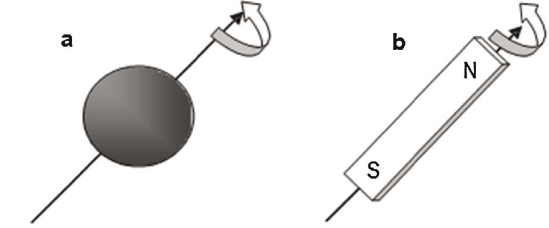
\includegraphics[width=0.5\textwidth]{Templates/Qualificacao/images/spin.png}
 \caption{\label{fig:spin_nuclei}Spin nuclear: O giro do núcleo ou \textit{spin} (a) induz um campo magnético, comportando-se como um imã (b). N e S representam o norte e o sul. A direção das setas representam a direção do campo magnético. Fonte: \citep{Grover2015}}
\end{figure}

\section{Fundamentos Teóricos} \label{ch:fundamentos}

Descreva aqui os principais conceitos e requisitos necessários para o desenvolvimento deste trabalho de mestrado.

\subsection{Exemplo Subseção} \label{sec:subsescao}

Para a melhor compreensão do funcionamento da aquisição de imagens por tensor de difusão (DTI) e a interpretação das sua medida de anisotropia fracionada (FA) é importante entender que a técnica de aquisição de imagens ponderadas por difusão (do inglês: \textit{Diffusion-weighted imaging} ou DWI) cujo modelo serve de base para fundamentar tanto as imagens por DTI quanto a técnica de fMRI. 

\subsubsection{Diffusion Imaging}

O fenômeno da difusão molecular é abordado no trabalho realizado por Einstein, em 1905,  que o explica com base no movimento randômico translacional das moléculas, que é resultante da sua energia termal \citep{Einstein}. 

\subsection{Anisotropia Fracionada (FA)}

A anisotropia Fracionada (FA) é uma medida adimensional do grau de “direcionalidade” da difusão intravoxel, ou seja, FA mede a “magnitude” da matriz de difusão, calculada por \citep{Pierpaoli}: 

\begin{equation}
FA=\frac{\sqrt{3}\sqrt{(\lambda_{1}-\lambda_{2})^{2}+(\lambda_{2}-\lambda_{3})^{2}+(\lambda_{3}-\lambda_{1})^{2}}}{\sqrt{2}\sqrt{\lambda_{1}^{2}+\lambda_{2}^{2}+\lambda_{3}^{2}}}
\label{eq:FA}
\end{equation}

\subsection{Atividades intrínsecas}

Biswal et al. \citep{biswal1995}  foram os primeiros a detectar, a nível de fMRI, que o “ruído” espontâneo do sinal BOLD exibia um padrão de coerência espacial nas regiões sensório-motoras no córtex cerebral (Figura \ref{f:restnet1}).

\begin{figure}[!htb]
    \centering
    \begin{subfigure}[b]{0.4\linewidth}        %% or \columnwidth
        \centering
        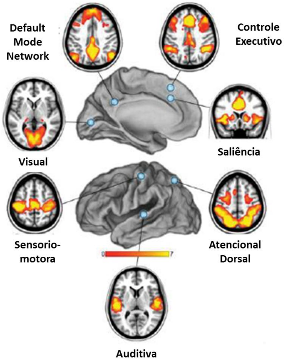
\includegraphics[width=\linewidth]{Qualificacao/images/restnet1.png}
        \caption{Principais redes de conectividade funcional em estado de repouso. Adaptado de \citeauthor{Raichle2011}, \citeyear{Raichle2011}.}
        \label{f:restnet1}
    \end{subfigure}\hfill
    \begin{subfigure}[b]{0.4\linewidth}        %% or \columnwidth
        \centering
        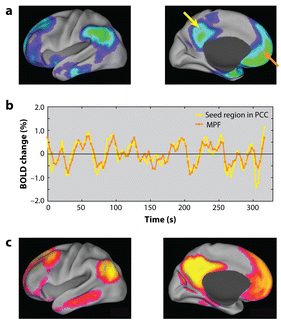
\includegraphics[width=\linewidth]{Qualificacao/images/restnet2.png}
        \caption{Visão da DMN na perspectiva de diminuição de atividade durante a performance de uma tarefa (a) e a conectividade funcional em estado de repouso (b e c). Adaptado de \citeauthor{Raichle2015}, \citeyear{Raichle2015}.}
        \label{f:restnet2}
    \end{subfigure}
    \caption{Representações da DMN. }
    \label{f:restnet}
\end{figure}

\section{Objetivos} \label{ch:objetivos}

Descreva aqui o objetivo central deste trabalho e detalhe o mesmo a partir de uma relação de objetivos específicos a serem alcançados.

Examplo de itemize:

\begin{itemize}

\item Objetivo 1;

\item Objetivo 2;

\item Objetivo 3.

\end{itemize}

Exemplo de itemize sem espaçamento:

\begin{itemize}
\setstretch{1}
\vskip0.2cm
\item Bullet 1
\item Bullet 2
\item Bullet 3
\end{itemize}

É importante salientar que cada objetivo específico deve ser seguido pela descrição da metodologia que será empregada para a sua realização.

\section{Proposta} \label{ch:metodologia}

Descreva aqui a proposta deste trabalho de mestrado. Entende-se por proposta o detalhamento do que será desenvolvimento durante o mestrado para garantir que o objetivo central deste trabalho seja alcançado.

\begin{figure}[!htb]
 \centering
 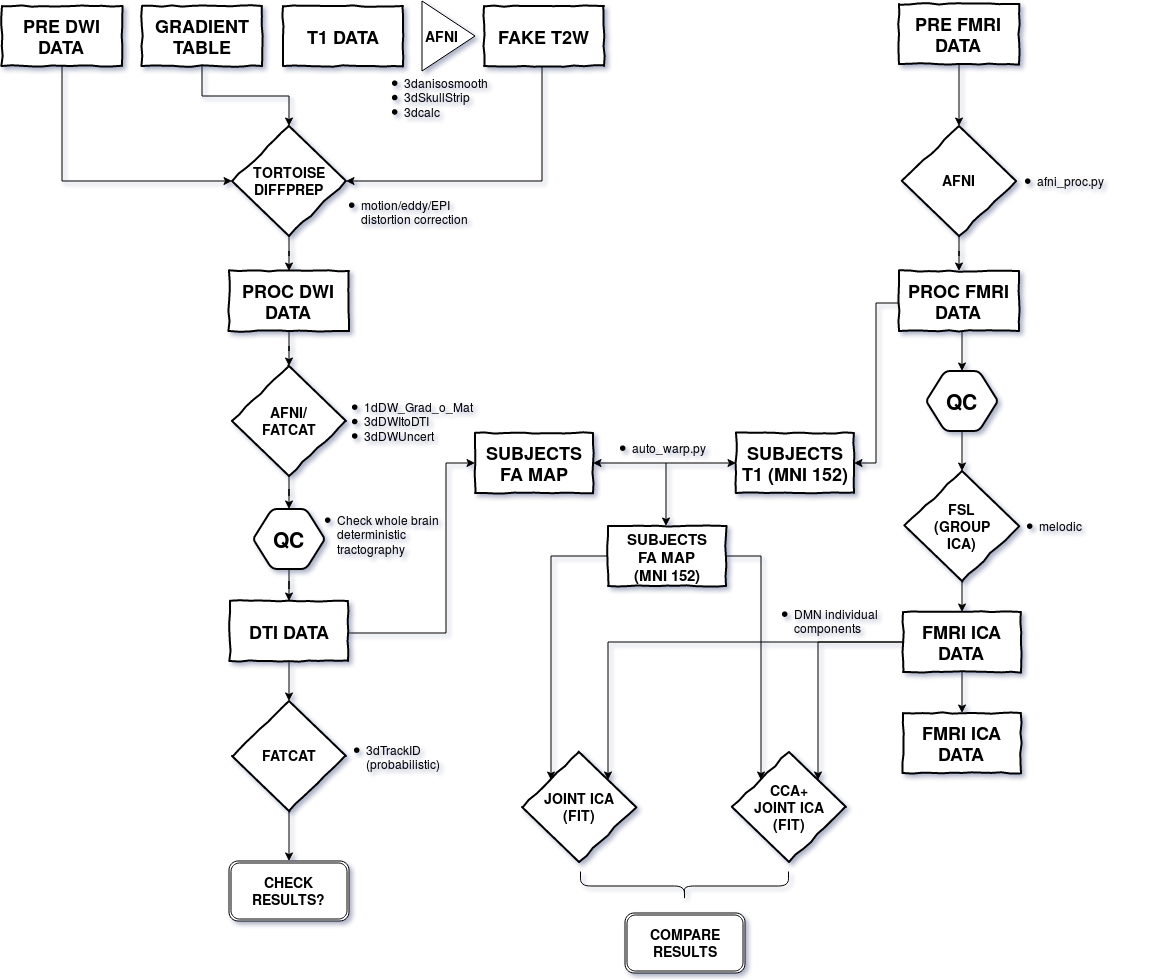
\includegraphics[width=0.9\textwidth]{Templates/Qualificacao/images/fluxograma.png}
 \caption{\label{fig:fluxograma}Exemplo de fluxograma (http://draw.io).}
\end{figure}

\section{Resultados e Discussão} \label{ch:simulacoes}

Inclua neste capítulo a descrição do Estudo de Caso e os resultados obtidos até o momento, se houverem. Além disso, inclua neste capítulo os resultados esperados. 

\section{Considerações Finais} \label{ch:consideracoes}

Descreva aqui as considerações finais sobre a proposta de Ante Projeto.  

\section{Cronograma} \label{ch:cronograma}

Insira aqui o cronograma a ser seguido durante a realização do trabalho. Observe que esse cronograma deve contemplar o período de 1 ano de trabalho até o término do curso de mestrado, ou seja, os últimos 12 meses de trabalho do aluno.

%O desenvolvimento do trabalho proposto está programado para cumprir as seguintes etapas:
Exemplo de um cronograma.
The development of the proposed work is scheduled to perform the following steps:

\begin{enumerate}
 \item Literature review;
 \item Study the pre-processing steps used for rs-fMRI;
 \item Study EMD method;
 \item Conducting simulations to validate the operation and robustness of the method;
 \item Writing qualification;
 \item Qualification defense;
 \item Correction of the noise level of signals acquired;
 \item Method application in task-based fMRI data;
 \item Method application in rs-fMRI data;
 \item Statistical analysis (correlation, multiple regression,...);
 \item Write journal paper;
 \item Dissertation writing;
 \item Dissertation defense;
\end{enumerate}

\definecolor{midgray}{gray}{.5}

\begin{table}[!htb]
\centering
\caption{Project schedule}
\label{my-label}
\begin{tabular}{l|l|l|l|l|l|l|l|l|l|l|}
\cline{2-11}
 & \multicolumn{9}{c|}{2015} & 2016 \\ \hline
\multicolumn{1}{|l|}{Step} & Apr & May & Jun & Jul & Aug & Sep & Oct & Nov & Dec & \multicolumn{1}{l|}{Jan} \\ \hline
\multicolumn{1}{|l|}{1} & \cellcolor{midgray} & \cellcolor{midgray} & \cellcolor{midgray} & \cellcolor{midgray} & \cellcolor{midgray} & \cellcolor{midgray} & \cellcolor{midgray} & \cellcolor{midgray} & \cellcolor{midgray} & \multicolumn{1}{l|}{\cellcolor{midgray}} \\ \hline
\multicolumn{1}{|l|}{2} & \cellcolor{midgray} &  &  &  &  &  &  &  &  & \multicolumn{1}{l|}{} \\ \hline
\multicolumn{1}{|l|}{3} &  & \cellcolor{midgray} &  &  &  &  &  &  &  & \multicolumn{1}{l|}{} \\ \hline
\multicolumn{1}{|l|}{4} &  &  & \cellcolor{midgray} & \cellcolor{midgray} &  &  &  &  &  & \multicolumn{1}{l|}{} \\ \hline
\multicolumn{1}{|l|}{5} &  &  & \cellcolor{midgray} & \cellcolor{midgray} &  &  &  &  &  & \multicolumn{1}{l|}{} \\ \hline
\multicolumn{1}{|l|}{6} &  &  &  &  & \cellcolor{midgray} &  &  &  &  & \multicolumn{1}{l|}{} \\ \hline
\multicolumn{1}{|l|}{7} &  &  &  &  & \cellcolor{midgray} &  &  &  &  & \multicolumn{1}{l|}{} \\ \hline
\multicolumn{1}{|l|}{8} &  &  &  &  & \cellcolor{midgray} & \cellcolor{midgray} &  &  &  & \multicolumn{1}{l|}{} \\ \hline
\multicolumn{1}{|l|}{9} &  &  &  &  &  & \cellcolor{midgray} & \cellcolor{midgray} &  &  & \multicolumn{1}{l|}{} \\ \hline
\multicolumn{1}{|l|}{10} &  &  &  &  &  &  &  & \cellcolor{midgray} &  & \multicolumn{1}{l|}{} \\ \hline
\multicolumn{1}{|l|}{11} &  &  &  &  &  &  & \cellcolor{midgray} & \cellcolor{midgray}  & \cellcolor{midgray} & \multicolumn{1}{l|}{\cellcolor{midgray}} \\ \hline
\multicolumn{1}{|l|}{12} &  &  &  &  &  &  &  & \cellcolor{midgray} & \cellcolor{midgray} & \multicolumn{1}{l|}{} \\ \hline
\multicolumn{1}{|l|}{13} &  &  &  &  &  &  &  &  &  & \multicolumn{1}{l|}{\cellcolor{midgray}} \\ \hline
\end{tabular}
\end{table}

\clearpage

% BIBLIOGRAFIA
\bibliographystyle{apa}
\setlength{\bibsep}{6pt}
\setstretch{1}
\bibliography{referencias}

\end{document}
